\chapter{Facility Details}

\section{Dimensions}
Based on the technical recommendation provided by FIFA, the official futsal playing pitch dimension should be $40m$ by $20m$. As the pitch is in an indoor facility, the ceiling height should be at least $6.1m$, as defined in~\cite{www:the_fa_guide}.

The facility must have a dimension of $185m \times 53m$ and the height is $8m$, so based on the futsal specification, the height of the ceiling is acceptable. The facility will have eight futsal pitches and the distance between each pitch will be of $3m$. The first and the last pitches will have their side distance between the wall and the pitch of $2m$. The distance from the goal line and the wall will be of $7.5m$. In order to retain the ball within the perimeters of pitch and to avoid disturbance of a concurrent game, a safety soccer net will also be installed between each pitch, the same will be installed behind each goal, which will protect the passages of other players.

The futsal ball has a size number $4$, which means its diameter is around $20cm$, therefore the work plan will be set at $20cm$ because the players have to keep an eye on the ball. Since the ceiling height recommendation is $6.1m$ and the facility's height is $8m$, the luminaires will be suspended at $50cm$ from the ceiling. The Figure~\ref{fig:cavity_dimensions} shows the work plan and the luminaires suspension height.

\begin{figure}[h!]
\centering
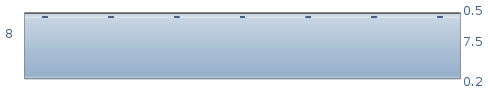
\includegraphics[width=.9\textwidth]{./figs/cavity_dimensions.png}
\caption{Facility's luminaires suspension height and work plan for futsal pitches.}
\label{fig:cavity_dimensions}
\end{figure}

\section{Operations}

The temperature of the facility is maintained between $20\degree$C and $25\degree$C throughout the entire year. This means that the lighting design will not have any corrective factor, thus the variations are very minimal.

During the calculus of the reflection, the floor will be assumed to be dirtier than the wall, because of the accumulated dust and the shoes tracks left by the players. The environment cleanness level is considered moderate because of the missing air filtration system.

Based on the fact gymnasiums commonly have light color walls and ceilings, this facility will follow this specification. For this type of environment the reflectance of the ceiling, wall and floor cavity will be $70\%$, $50\%$ and $20\%$, respectively.

Such as a common facility, the voltage to be utilized in this facility is set at $120V$.

